\documentclass[aspectratio=169]{../latex_main/tntbeamer}  % you can pass all options of the beamer class, e.g., 'handout' or 'aspectratio=43'
\usepackage{dsfont}
\usepackage{bm}
\usepackage[english]{babel}
\usepackage[T1]{fontenc}
%\usepackage[utf8]{inputenc}
\usepackage{graphicx}
\graphicspath{ {./figures/} }
\usepackage{algorithm}
\usepackage[ruled,vlined,algo2e,linesnumbered]{algorithm2e}
\usepackage{hyperref}
\usepackage{booktabs}
\usepackage{mathtools}

\usepackage{amsmath,amssymb}

\DeclareMathOperator*{\argmax}{arg\,max}
\DeclareMathOperator*{\argmin}{arg\,min}

\usepackage{amsbsy}
\newcommand{\vect}[1]{\bm{#1}}
%\newcommand{\vect}[1]{\boldsymbol{#1}}

\usepackage{pgfplots}
\pgfplotsset{compat=1.16}
\usepackage{tikz}
\usetikzlibrary{trees} 
\usetikzlibrary{shapes.geometric}
\usetikzlibrary{positioning,shapes,shadows,arrows,calc,mindmap}
\usetikzlibrary{positioning,fadings,through}
\usetikzlibrary{decorations.pathreplacing}
\usetikzlibrary{intersections}
\pgfdeclarelayer{background}
\pgfdeclarelayer{foreground}
\pgfsetlayers{background,main,foreground}
\tikzstyle{activity}=[rectangle, draw=black, rounded corners, text centered, text width=8em]
\tikzstyle{data}=[rectangle, draw=black, text centered, text width=8em]
\tikzstyle{myarrow}=[->, thick, draw=black]

% Define the layers to draw the diagram
\pgfdeclarelayer{background}
\pgfdeclarelayer{foreground}
\pgfsetlayers{background,main,foreground}

% Requires XeLaTeX or LuaLaTeX
%\usepackage{unicode-math}

\usepackage{fontspec}
%\setsansfont{Arial}
\setsansfont{RotisSansSerifStd}[ 
Path=../latex_main/fonts/,
Extension = .otf,
UprightFont = *-Regular,  % or *-Light
BoldFont = *-ExtraBold,  % or *-Bold
ItalicFont = *-Italic
]
\setmonofont{Cascadia Mono}[
Scale=0.8
]

% scale factor adapted; mathrm font added (Benjamin Spitschan @TNT, 2021-06-01)
%\setmathfont[Scale=1.05]{Libertinus Math}
%\setmathrm[Scale=1.05]{Libertinus Math}

% other available math fonts are (not exhaustive)
% Latin Modern Math
% XITS Math
% Libertinus Math
% Asana Math
% Fira Math
% TeX Gyre Pagella Math
% TeX Gyre Bonum Math
% TeX Gyre Schola Math
% TeX Gyre Termes Math

% Literature References
\newcommand{\lit}[2]{\href{#2}{\footnotesize\color{black!60}[#1]}}

%%% Beamer Customization
%----------------------------------------------------------------------
% (Don't) Show sections in frame header. Options: 'sections', 'sections light', empty
\setbeamertemplate{headline}{empty}

% Add header logo for normal frames
\setheaderimage{
	% 
\includegraphics[height=\logoheight]{figures/TNT_darkv4.pdf}
	
\includegraphics[height=\logoheight]{../latex_main/figures/luh_logo_rgb_0_80_155.pdf}
	% 
\includegraphics[height=\logoheight]{figures/logo_tntluh.pdf}
}

% Header logo for title page
\settitleheaderimage{
	% 
\includegraphics[height=\logoheight]{figures/TNT_darkv4.pdf}
	
\includegraphics[height=\logoheight]{../latex_main/figures/luh_logo_rgb_0_80_155.pdf}
	% 
\includegraphics[height=\logoheight]{figures/logo_tntluh.pdf}
}

% Title page: tntdefault 
\setbeamertemplate{title page}[tntdefault]  % or luhstyle
% Add optional title image here
%\addtitlepageimagedefault{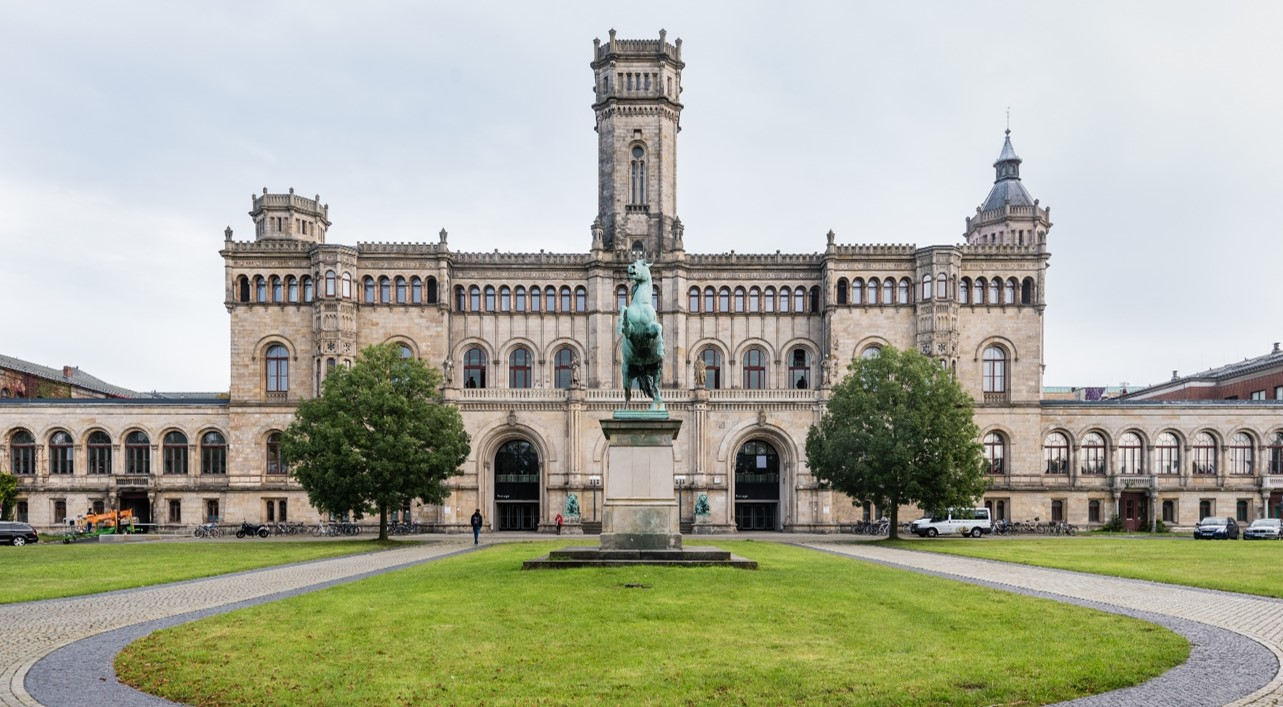
\includegraphics[width=0.65\textwidth]{figures/luh_default_presentation_title_image.jpg}}

% Title page: luhstyle
% \setbeamertemplate{title page}[luhstyle]
% % Add optional title image here
% \addtitlepageimage{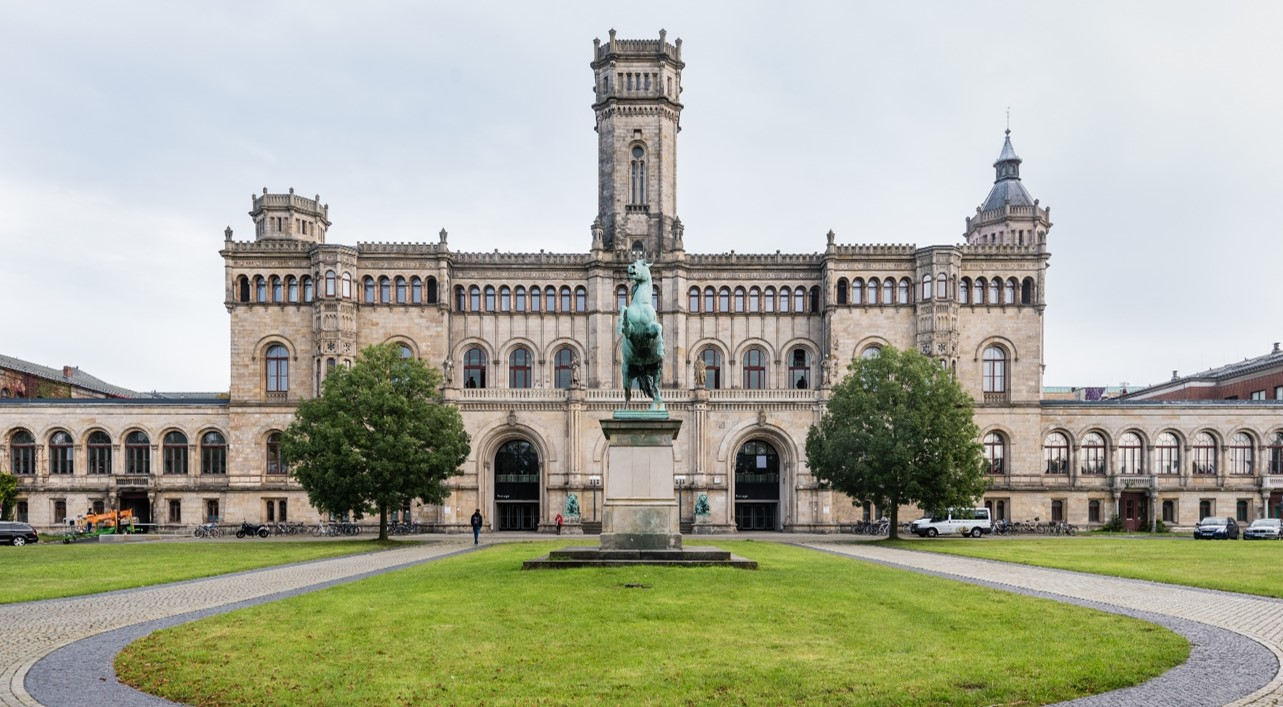
\includegraphics[width=0.75\textwidth]{figures/luh_default_presentation_title_image.jpg}}

\author[Abedjan \& Lindauer]{Ziawasch Abedjan \& Marius Lindauer\\[1em]
	
\includegraphics[height=\logoheight]{../latex_main/figures/luh_logo_rgb_0_80_155.pdf}\qquad
	
\includegraphics[height=\logoheight]{../latex_main/figures/DBIS_Kurzlogo.png}\qquad

\includegraphics[height=\logoheight]{../latex_main/figures/TNT_darkv4}\qquad

\includegraphics[height=\logoheight]{../latex_main/figures/L3S.jpg}	}
\date{Summer Term 2022; \hspace{0.5em} {
\includegraphics[height=1.5em]{../latex_main/figures/Cc-by-nc-sa_icon.svg.png}}; based on \href{https://ds100.org/fa21/}{[DS100]}
}


%%% Custom Packages
%----------------------------------------------------------------------
% Create dummy content
\usepackage{blindtext}

% Adds a frame with the current page layout. Just call \layout inside of a frame.
\usepackage{layout}


%%% Macros
%\renewcommand{\vec}[1]{\mathbf{#1}}
% \usepackage{bm}
%\let\vecb\bm

\title[Introduction]{DS: Gradient Descent}
\subtitle{Stochastic Gradient Descent}

\graphicspath{ {./figure/} }
%\institute{}


\begin{document}
	
	\maketitle
	\begin{frame}{The Gradient Descent Algorithm}
	    \vspace{1cm}
	    \hspace{4cm}\fbox{\parbox{.4\textwidth}{$\theta^{(0)} \leftarrow$ initial vector (random, zeros …)\\
	    For $\tau$ from 0 to convergence:\\
	    \begin{equation*}
	         \Vec{\theta}^{(t+1)} = \Vec{\theta}^{(t)} - \alpha \nabla_{\Vec{\theta}}L(\Vec{\theta}, \mathbb{X}, \Vec{y})
	    \end{equation*}}}
	    \begin{itemize}
	        \item $\alpha$ is the learning rate
	        \item Converges when gradient is $\approx$ 0 (or we run out of patience)
	    \end{itemize}
	\end{frame}
	
	
	\begin{frame}{Which Step in This Algorithm is Most Time Consuming?}
    	Gradient Descent Algorithm\\
    	\vspace{1cm}
	    \hspace{4cm}\fbox{\parbox{.4\textwidth}{$\theta^{(0)} \leftarrow$ initial vector (random, zeros …)\\
	    For $\tau$ from 0 to convergence:\\
	    \begin{equation*}
	         \Vec{\theta}^{(t+1)} = \Vec{\theta}^{(t)} - \alpha \fcolorbox{red}{white}{\parbox{.13\textwidth}{$\nabla_{\Vec{\theta}}L(\Vec{\theta}, \mathbb{X}, \Vec{y}$)}}
	    \end{equation*}}}
	\end{frame}
	
	
	
	\begin{frame}{Which Step in This Algorithm is Most Time Consuming?}
	    \begin{equation*}
	         \Vec{\theta}^{(t+1)} = \Vec{\theta}^{(t)} - \alpha \fcolorbox{red}{white}{\parbox{.13\textwidth}{$\nabla_{\Vec{\theta}}L(\Vec{\theta}, \mathbb{X}, \Vec{y}$)}}
	    \end{equation*}
	    Typically the loss function is really the average loss over a large dataset.
	    \begin{equation*}
	        \nabla_\theta L(\theta)  \left|_{\theta = \theta^{(\tau)}}=\frac{1}{n}\sum_{i=1}^n \nabla_\theta \text{loss}(y,f_\theta (x))\right|_{\theta = \theta^{(\tau)}}
	    \end{equation*}
	    \begin{itemize}
	        \item Loading and computing on all the data is expensive.
	        \item What do we do when accessing the “population” is prohibitively expensive?
	    \end{itemize}
	\end{frame}
	
	
	
	\begin{frame}{Stochastic Gradient Descent}
    	\vspace{0cm}
	    \hspace{4cm}\fbox{\parbox{.5\textwidth}{$\theta^{(0)} \leftarrow$ initial vector (random, zeros …)\\
	    For $\tau$ from 0 to convergence:\\
	    \vspace{.1cm}
	    \hspace{1cm}
	    $\mathcal{B} \textasciitilde $Random subset of indices\\
	    \begin{equation*}
	        \theta^{(\tau + 1)} \leftarrow \theta^{(\tau)} -  \alpha\left(\left.\frac{1}{|\mathcal{B}|}\sum\limits_{i\in \mathcal{B}}\nabla_\theta L_i(\theta)\right|_{\theta = \theta^{(\tau)}}\right)
	    \end{equation*}}}
	    \begin{itemize}
	        \item[1.] Draw a simple random sample of data indices 
	        \begin{itemize}
	            \item Often called a batch or mini-batch
	            \item Choice of batch size trade-off gradient quality and speed
	        \end{itemize}
	        \item[1.] Compute gradient estimate and uses as gradient
	    \end{itemize}
	\end{frame}
	
	
	
	\begin{frame}{Stochastic Gradient Descent}
    	\vspace{0cm}
	    \hspace{4cm}\fbox{\parbox{.5\textwidth}{$\theta^{(0)} \leftarrow$ initial vector (random, zeros …)\\
	    For $\tau$ from 0 to convergence:\\
	    \vspace{.1cm}
	    \hspace{1cm}
	    $\mathcal{B} \textasciitilde $Random subset of indices\\
	    \begin{equation*}
	        \theta^{(\tau + 1)} \leftarrow \theta^{(\tau)} -  \alpha\left(\left.\frac{1}{|\mathcal{B}|}\sum\limits_{i\in \mathcal{B}}\nabla_\theta L_i(\theta)\right|_{\theta = \theta^{(\tau)}}\right)
	    \end{equation*}}}\\
	   Decomposable Loss
       \begin{equation*}
           L(\theta)  = \sum\limits_{i=1}^nL_i(\theta) = \sum\limits_{i=1}^nL(\theta, x_i, y_i)
       \end{equation*}
       Loss can be written as a sum of the loss on each record.
	\end{frame}
	
	
	
	\begin{frame}{.}
	    \vspace{-1cm}
	    \hspace{2cm}\fbox{\parbox{.7\textwidth}{$\theta^{(0)} \leftarrow$ initial vector (random, zeros …)\\
	    For $\tau$ from 0 to convergence:\\
	    \begin{equation*}
	        \theta^{(\tau + 1)} \leftarrow \theta^{(\tau)} -  \alpha\left(\left.\frac{1}{n}\sum\limits_{i=1}^n\nabla_\theta L_i(\theta)\right|_{\theta = \theta^{(\tau)}}\right)
	    \end{equation*}}}
        
        \vspace{1cm}
	    \hspace{2cm}\fbox{\parbox{.7\textwidth}{$\theta^{(0)} \leftarrow$ initial vector (random, zeros …)\\
	    For $\tau$ from 0 to convergence:\\
	    \vspace{.1cm}
	    \hspace{1cm}
	    $\mathcal{B} \textasciitilde $Random subset of indices\\
	    \begin{equation*}
	        \theta^{(\tau + 1)} \leftarrow \theta^{(\tau)} -  \alpha\left(\left.\frac{1}{|\mathcal{B}|}\sum\limits_{i\in \mathcal{B}}\nabla_\theta L_i(\theta)\right|_{\theta = \theta^{(\tau)}}\right)
	    \end{equation*}}}\\
       
       \vspace{-3.6cm}
       \hspace{8.5cm}
\includegraphics[scale=.4]{Bild29}\\
       \hspace{3.6cm}
       
       \vspace{-5.8cm}
       \hspace{1.5cm}\rotatebox{90}{Gradient Descent}\\
       \vspace{5.8cm}
       
       \vspace{-5.3cm}
       \hspace{1.5cm}\rotatebox{90}{Stochastic Gradient Descent}\\
       \vspace{5.3cm}
       
       \vspace{-12.5cm}
       \hspace{12.8cm}\rotatebox{270}{Assuming Decomposable Loss Functions}\\
       \vspace{12.5cm}
	\end{frame}
	
	
	\begin{frame}{Gradient Descent}
	    \vspace{-.5cm}
	    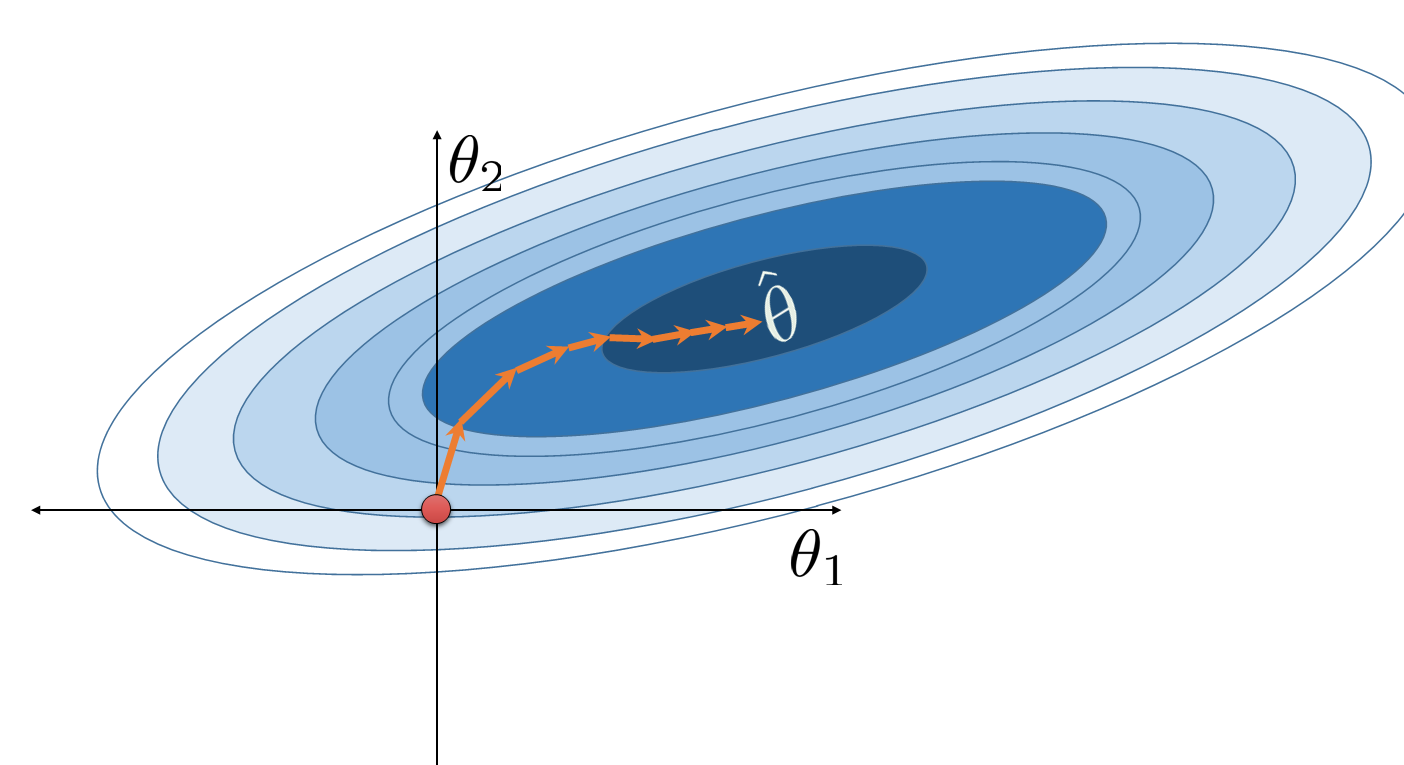
\includegraphics[scale=.4]{Bild30}
	\end{frame}
	
	
	
	\begin{frame}{\underline{Stochastic} Gradient Descent}
	    \vspace{-.5cm}
        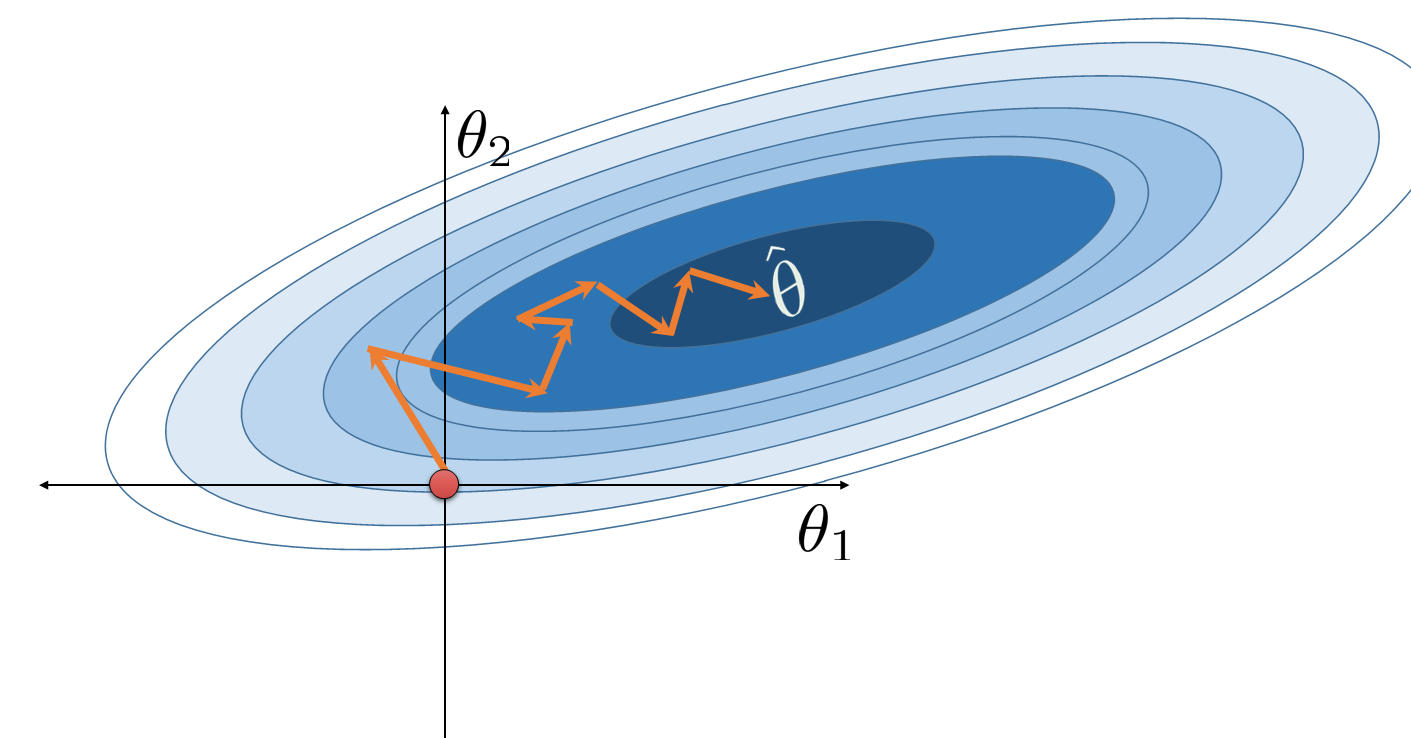
\includegraphics[scale=.4]{Bild31}
	\end{frame}
\end{document}